\documentclass[11pt]{article}
\usepackage{geometry}                % See geometry.pdf to learn the layout options. There are lots.
\geometry{a4paper}                   % ... or a4paper or a5paper or ... 
\usepackage{graphicx}
\usepackage{amssymb}
\usepackage{url}
\usepackage{listings}
\usepackage{color}

\renewcommand{\textfraction}{0.15}
\renewcommand{\topfraction}{0.85}
\renewcommand{\bottomfraction}{0.65}
\renewcommand{\floatpagefraction}{0.60}

\lstset{ %
language=C++,                  %choose the language of the code
basicstyle=\footnotesize\ttfamily,% the size of the fonts that are used for the code
showstringspaces=false,         % underline spaces within strings
numbers=left,                   % where to put the line-numbers
numberstyle=\ttfamily,      % the size of the fonts that are used for the line-numbers
stepnumber=2,                   % the step between two line-numbers. If it's 1 each line will be numbered
numbersep=5pt,                  % how far the line-numbers are from the code
stringstyle=\ttfamily,          % typewriter type for strings
backgroundcolor=\color{white},  % choose the background color
showspaces=false,               % show spaces within strings adding particular underscores
showtabs=false,                 % show tabs within strings adding particular underscores
escapeinside={\%*}{*)},         % if you want to add a comment within your code
breaklines=true,                 % break line if it is too long
frame=leftline
}

\usepackage{fontspec,xltxtra,xunicode}
\defaultfontfeatures{Mapping=tex-text}
\setromanfont[Mapping=tex-text]{Georgia}
\setsansfont[Scale=MatchLowercase,Mapping=tex-text]{Tahoma}
\setmonofont[Scale=MatchLowercase]{Courier New}


\title{IEG4180 Project 2\\NetProbe Documentation}
\author{GUAN Hao\\05569511\\hguan5@ie.cuhk.edu.hk}
\date{\today}
\begin{document}
\maketitle
\section{Introduction}
In this project, I write both a server and a client for the NetProbe.

The NetProbe Server will listen for incoming connections roiginating from a NetProbe Client, receiving the operating parameters and transmit packets. It is a concurrent server which is implemented using select-base I/O multiplexing.

The NetProbe Client is based on the last version in Project 1 and Message-Driven I/O mode is added in this version. User can choose either {\em TCP} or {\em UDP} protocol and either {\em Blocking} or {\em Message-Driven} I/O mode to receive the packets. The same as the last version, operating parameters can be set can the transmission statistics will be updated according to the sepecified refresh interval.
\section{Program Structure}
The program is a MFC application which is designed with the Object-Oriented concept. Following is the list of classes implemented in this project:
\subsection{NetProbe Server}
There is only one class in the server side.
\begin{itemize}
\item {\tt class NetProbeServer}, the main class of the NetProbe Server. This class will initialize the TCP and UDP sockets, use {\tt select()} to detect the protocol of the incomming connection and start new threads to send packets. Following is the prototype of this class.  
\begin{lstlisting}
class NetProbeServer{
private: 
	struct sockaddr_in *TCP_Addr;
	struct sockaddr_in *UDP_Addr;
	struct sockaddr_in *createSockAddr(char *host, int port);
	SOCKET tcpfd, udpfd;

public:
	NetProbeServer(const char *tcp_h, int tcp_p, const char *udp_h, int udp_p);
	int TCPReady(void);
	int UDPReady(void);
	int detectProtocol(void);
	static DWORD WINAPI threadTCPSend(LPVOID lpInstance);
	static DWORD WINAPI threadUDPSend(LPVOID lpInstance);
};
\end{lstlisting}
\end{itemize}
\subsection{NetProbe Client}
\begin{itemize}
\item {\tt class CNetProbeClinetApp}, the main class of this program. This class will create a instance of {\tt class CNetProbeDlg} and show the dialog. Some {\tt winsock} initialize functions are also invoked here.
\item {\tt class CNetProbeClientDlg}, this class control the main dialog of the application. 
\item {\tt class NetProbe}, all the socket operation is implemented in this class. Following shows the prototype of {\tt class NetProbe}:
\begin{lstlisting}
class NetProbe
{
private: 
	struct sockaddr_in *Server_Addr;
	struct sockaddr_in *createSockAddr(char *host, int port);
	SOCKET Sockfd;
	CNetProbeClientDlg *theDlg;
	double bytesTransferred;
	int packetsTransferred;
	int maxPacketNum;
	ES_FlashTimer timer;
	int status;
	int PacketSize;
	int SendingRate;
	int NumPackets;


public:
	NetProbe(CNetProbeClientDlg *dialog, char *host, int port);
	CWinThread *wThread;
	void stop();
	static DWORD WINAPI threadUpdateUI(LPVOID lpInstance);
	int TCPConnect(LPVOID lpInstance);
	static DWORD WINAPI threadTCPReceive(LPVOID lpInstance);
	int UDPConnect(LPVOID lpInstance);
	static DWORD WINAPI threadUDPReceive(LPVOID lpInstance);
	int MsgDrivenReady();
	void OnRead();
	void OnClose();
	
};
\end{lstlisting}
\end{itemize}
\section{GUI Design}
There is no GUI for the NetProbe Server and for NetProbe Client a similar GUI with the last version is used.
\begin{figure}
\centering
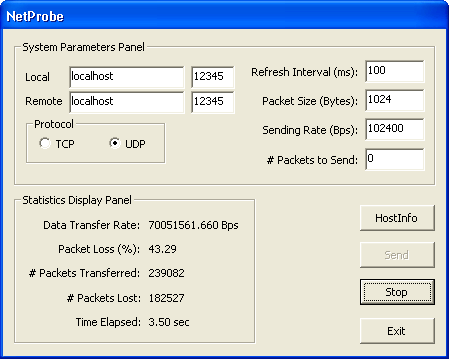
\includegraphics[width=3in]{work.png}
\caption{Statistics shown on the dialog.}
\label{fig:work}
\end{figure}
The main dialog is designed as in Figure \ref{fig:work}. User can input parameters and choose protocol on this dialog.After {\em Send} or {\em Receive} button is clicked, the caption of the button will turn to {\em Stop}. During transmission, the statistics will be shown on the bottom of the dialog.

\end{document}
